% vim:set spell:
% vim:spell spelllang=fr:
\documentclass[a4paper]{article}
\usepackage[utf8x]{inputenc}
\usepackage[T1]{fontenc}
\usepackage{charter}
\usepackage{helvet}
\usepackage{graphicx}
\usepackage{amsmath,amssymb}
\usepackage[french]{babel}
\usepackage{xspace}
\usepackage{setspace}
\setstretch{1.0}
\usepackage{subfigure}
\voffset       -1in
\hoffset       -1in
\headheight     12pt
\headsep        12pt
\topmargin      25mm
\oddsidemargin  20mm
\textwidth      170mm
\textheight     240mm
\flushbottom

\begin{document}
\begin{center}
\large
Travaux Pratiques Archi SLE-3A\\
Cours de Frédéric Pétrot\\
\LARGE
Implantations et évaluations de\\
quelques prédicteurs de branchements\\
\large

Durée~: 3 heures
\end{center}
\section{Organisation}
Attention, le travail demandé dans ce TP doit faire l'objet d'un court rapport qui inclut les \emph{sources} des prédicteurs et les \emph{résultats} d'expérimentations à fournir en fin de séance.
Un gabarit en \LaTeX\ qui reprend le predicteur 1-bit donné en exemples et quelques scripts sont fournis pour vous permettre de le faire vite, il est néanmoins nécessaire de réserver au moins 20 minutes pour consolider vos écrits.
Vous avez intérêt à ajouter vos résultats au fur et à mesure.

\section{Introduction}
On cherche à étudier le comportement en situation réelle de différents prédicteurs.
Pour cela, on va développer un modèle en C++ de chacun de ces prédicteurs sur lequel on fera passer un ensemble de traces d'exécutions et qui fournira en sortie le ratio de mauvaises prédictions (en fait le nombre de \emph{Miss Prediction per Kilo (Branch) Instructions}, MPKI).
On fera varier les différents paramètres du prédicteur, en particulier la taille des tables, afin d'en extraire un comportement asymptotique (par benchmark), dont on tirera un graphe.

L'infrastructure dans laquelle insérer le modèle de prédicteur est celle qui a été utilisée par le \emph{The 2nd JILP Championship Branch Prediction Competition (CBP-2)}\footnote{\texttt{http://cava.cs.utsa.edu/camino/cbp2/}}.
Cette infrastructure effectue la lecture des traces et l'appel à des fonctions qui implantent le prédicteur, et donne en sortie uniquement la valeur du MPKI.


Le prédicteur par défaut dans l'archive est le prédicteur «~1-bit~» vu en cours et rappelé figure~\ref{1-bit}.
Nous ferons une analyse rapide en séance afin de comprendre comment implanter un prédicteur dans l'infrastructure.
\begin{figure}[hbt]\center\leavevmode
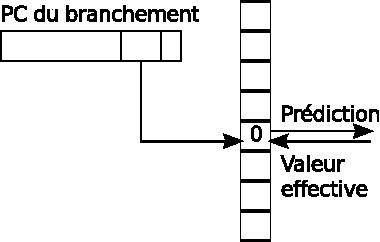
\includegraphics[scale=.9]{1-bit}
\caption{Prédicteur 1-bit}
\label{1-bit}
\end{figure}
Un branchement pris (ou prédit pris) sera à \verb+true+ (ou encore $1$ si considéré comme un bit) et non pris (ou prédit non pris) sera à \verb+false+ (ou encore $0$ si considéré comme un bit).

\section{Travail demandé}
On implantera différents prédicteurs en prenant soin de paramétrer les tailles afin de pouvoir lancer facilement plusieurs exécutions (\emph{cf.} l'exemple fourni) et ainsi pouvoir tracer des courbes et voir les asymptotes.

Les prédicteurs que l'on pourra d'implanter sont les suivants~:
\begin{enumerate}
\item un prédicteur bimodal à 4 états dont le principe est illustré
      sur la figure~\ref{2-bits}.
      \begin{figure}[hbt]\center\leavevmode
      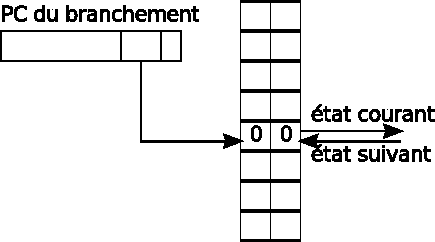
\includegraphics[scale=1]{2-bits}
      \caption{Prédicteur bimodal}
      \label{2-bits}
      \end{figure}
      
      On fera l'expérience avec le graphe de transitions vu en cours et rappelé ci-après.
      \begin{figure}[htb]
      \center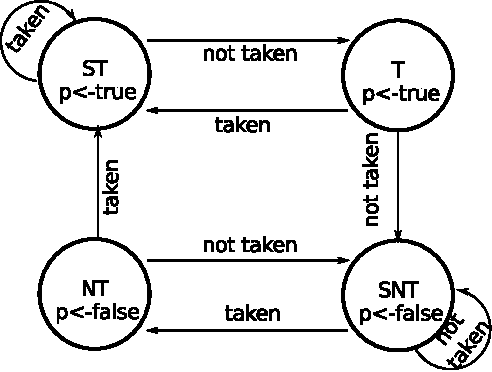
\includegraphics[scale=.6]{2bg1}
      \caption{\label{graphes}Graphe de transitions du prédicteur bimodal}
      \end{figure}

\item un prédicteur global simple avec un historique des branchement de longueur (nombre de bits) $H$ permettant d'atteindre une entrée bimodale utilisant le graphe d'état n°1 (la \emph{Pattern History Table}).
      Pour mémoire, l'historique des branchements est un registre à décalage à gauche dans lequel on injecte sur le poids faible la décision prise ($H=3$ dans la figure~\ref{global-simple}).
      \begin{figure}[hbt]\center\leavevmode
      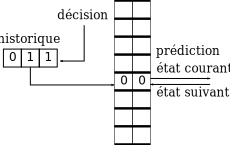
\includegraphics[scale=.9]{global-simple}
      \caption{Prédicteur global simple}
      \label{global-simple}
      \end{figure}

\item un prédicteur \emph{gshare} qui est un prédicteur global pour lequel l'index définissant l'entrée dans la table de taille $2^n$ est calculé comme le ou-exclusif d'un registre d'historique avec le pc du branchement, comme illustré sur la figure~\ref{gshare}.
      \begin{figure}[hbt]\center\leavevmode
      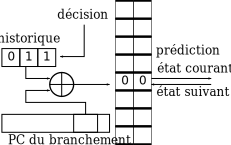
\includegraphics[scale=.9]{gshare}
      \caption{Prédicteur \emph{gshare}}
      \label{gshare}
      \end{figure}
      Si $H>n$, alors on prendra les $n$ bits de poids fort de $H$ pour faire le ou-exclusif.

\item un prédicteur corrélé qui utilise un historique sur $H$ bits permettant de sélectionner une PHT parmi $2^H$ et utilisant l'adresse du branchement pour indicer cette table, comme illustré sur la figure~\ref{correlated}.
      \begin{figure}[hbt]\center\leavevmode
      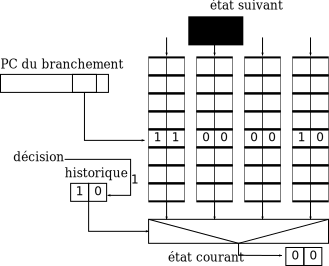
\includegraphics[scale=.9]{correlated}
      \caption{\label{correlated}Prédicteur corrélé}
      \end{figure}

\item un prédicteur local qui utilise une table d'historiques sur $H$ bits indexée par les poids faibles de l'adresse du branchement.  En utilisant l'entrée d'historique, on indice une PHT bimodale de taille $2^H$, comme illustré sur la figure~\ref{local}.
      \begin{figure}[hbt]\center\leavevmode
      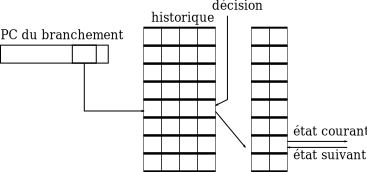
\includegraphics[scale=.9]{local}
      \caption{Prédicteur local}
      \label{local}
      \end{figure}

\item et pour finir un prédicteur mixte (celui de l'alpha 21264) qui utilise un prédicteur global simple avec un historique de $H_g=12$ (soit 4096 entrées), et un prédicteur local comme celui de la précédente question, avec $H_l=10$ par entrée de la table d'historique (soit 1024 entrées).
      La PHT indexée est un simple prédicteur de type bimodale, mais sur 3 bits, implantée avec un compteur à saturation (comme celle du graphe n°3 de la figure~\ref{graphes}).

      Le choix du prédicteur à utiliser se fait grâce à une BHT de 4K entrées de 2 bits.
      Le compteur est incrémenté lorsque le prédicteur \emph{prédit} est correcte et l'autre prédicteur a fait le mauvais choix, et est décrémenté dans le cas opposé (\emph{cf.} la machine d'état de la figure~\ref{mixte-graphe}).
      \begin{figure}[hbt]\center\leavevmode
      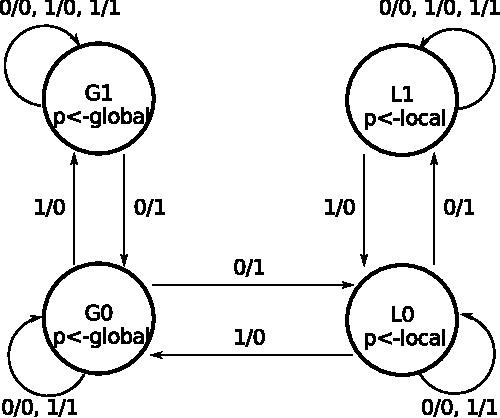
\includegraphics[scale=0.7]{mixte-graphe}
      \caption{Machine à états du choix du prédicteur.
      Légende~: $global/local$, $0$ décision incorrecte, $1$ décision correcte}
      \label{mixte-graphe}
      \end{figure}

      On ne tentera pas (du moins dans le temps imparti) de faire une version paramétrable de ce dernier prédicteur.
\end{enumerate}

Il y a un script \verb+run+ à la racine qui lance automatiquement l'exécution sur la totalité des traces pour un prédicteur donné, dont le nom de guerre est passé en premier argument sur la ligne de commande.
Il y a dans le script 3 boucles imbriquées~: la boucle externe, indice $k$ fait varier la longueur de l'historique ($k$ ne prend qu'une valeur quelconque pour les prédicteurs n'ayant pas d'historique), la boucle du milieu, d'indice $j$, fait varier le nombre de bits de PC à utiliser pour indexer les tables, et la boucle interne, d'indice $i$, elle, parcours l'ensemble des traces.
Vous serez amené à modifier les valeurs des bornes en fonction des prédicteurs, voir à changer un peu cette partie si vous faite des prédicteurs exotiques.

Le script \verb+run+ crée deux répertoires par prédicteur, l'un contenant les résultats l'autre les figures.

Afin de paramétrer simplement le prédicteur (sans avoir à toucher à l'infrastructure), on inclura (\verb+#include+) le prédicteur  comme unique fichier dans \verb+my_predictor.h+), les temps de compilation étant très faibles%
\footnote{\texttt{time ./run} donne \texttt{267,91s user 9,73s system 117\% cpu 3:55,91 total}}.

On utilisera \verb+gnuplot+ avec le script \verb+plot+ pour obtenir les courbes. 
On donne sur la figure~\ref{results} le type de résultat attendu pour le prédicteur 1 bit.

      \begin{figure}[htb]
      \centering
      \subfigure[Graphes 0 à 4]{
      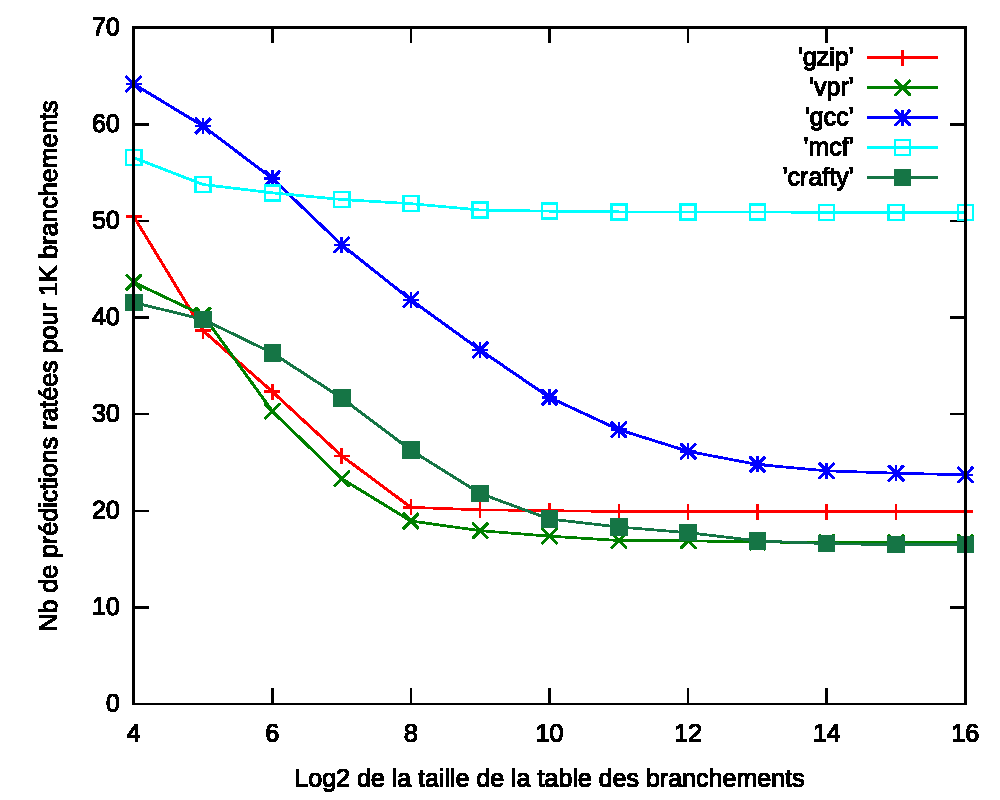
\includegraphics[scale=.48]{1-bit-0}
      \label{plot1}
      }
      \subfigure[Graphes 5 à 9]{
      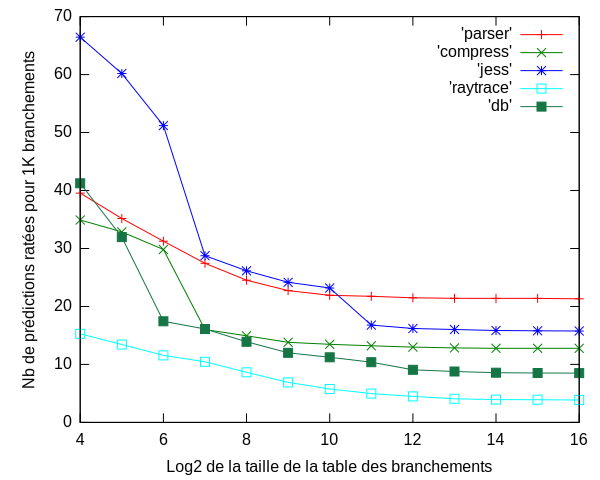
\includegraphics[scale=.48]{1-bit-1}
      \label{plot2}
      }
      \subfigure[Graphe 10 à 14]{
      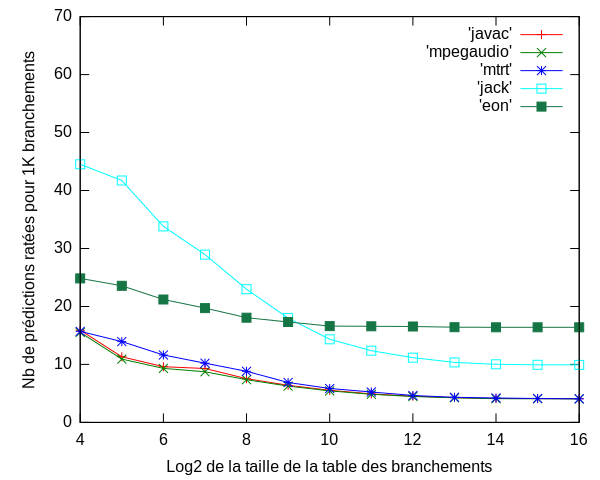
\includegraphics[scale=.48]{1-bit-2}
      \label{plot3}
      }
      \subfigure[Graphe 15 à 19]{
      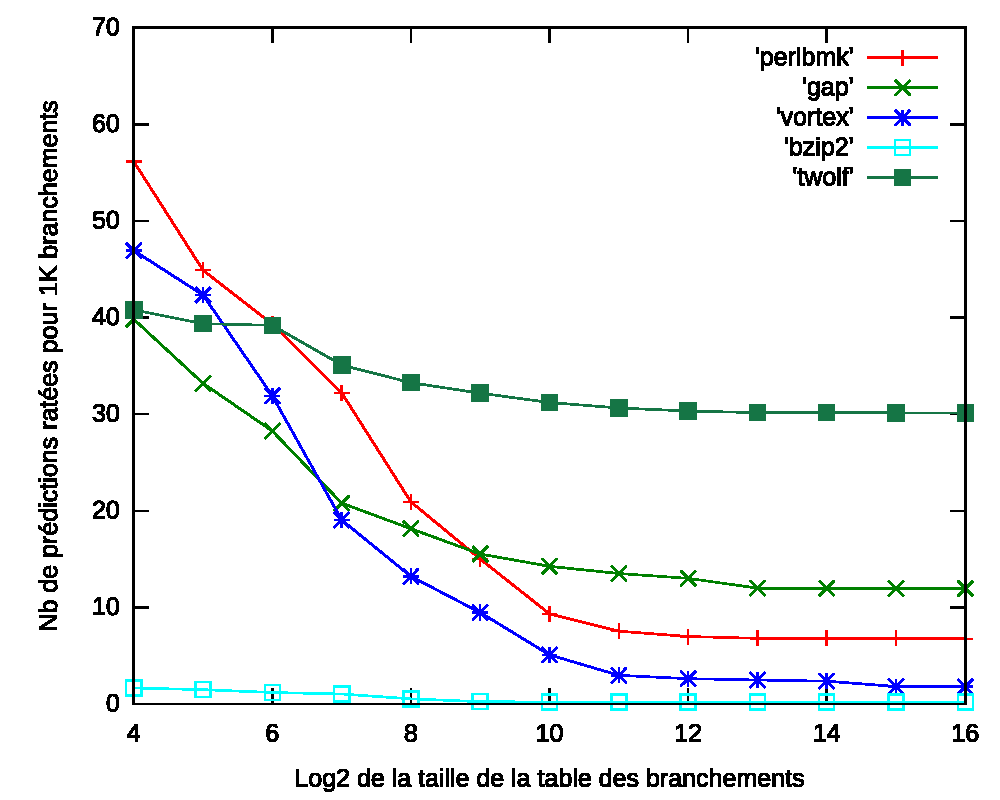
\includegraphics[scale=.48]{1-bit-3}
      \label{plot4}
      }
      \caption{\label{results}Les courbes de MPKI}
      \end{figure}

Le sous-répetoire \verb+rendu+ contient un exemple de .tex permettant de faire un petit rapport sur le travail.
\end{document}
